\chapter{Background} \label{chapter:part1-background}
\graphicspath{{Part1/Background/figures/}}

\section{Semantic Web} \label{section:sematic-web}

The web can be seen as a worldwide, distributed system of interconnected documents that humans can read, exchange and discuss. The original model behind the web can be roughly summarized as a way to publish documents represented in a standard form (e.g., HTML), containing links to other documents accessible through standard protocols (e.g., HTTP).

The great advantage of the web is that it abstracts the physical storage and network layers involved in the information exchange between machines. This enables documents to appear directly connected to one another. However, in this paradigm machines are not able to achieve tasks based on automated data processing such as search and query answering. To overcome this limitation, research fields such as Information Retrieval (IR), Machine Learning (ML), and Natural Language Processing (NLP) produced complex systems trying to automatically extract meaning from unstructured data. A typical example would be search engines such as Yahoo\footnote{\url{http://www.yahoo.com}} and Google\footnote{\url{http://www.google.com}}. Despite their success, there is still a semantic gap between what the machine understands and how the user perceives the data~\cite{Mika:book:07}. This is where Semantic Web intervenes trying to fill the knowledge gap. In the same way that original Web abstracted away the network and physical layers, the Semantic Web abstracts away the document and application layers involved in the exchange of information. The Semantic Web connects facts, so that rather than linking to a specific document or application, you can instead refer to a specific piece of information contained in that document or application. Berners-Lee et al.~\cite{BernersLee:ScientificAmerican:01} provide the following definition for the Semantic Web:

\begin{quote}
	\emph{The Semantic Web is not a separate Web but an extension of the current one, in which information is given well-defined meaning, better enabling computers and people to work in cooperation.}
\end{quote}

The word ``semantic'' itself implies meaning or understanding. The fundamental difference between Semantic Web and other data-related technologies is that the Semantic Web is concerned with the meaning and not the structure of data. This fundamental difference engenders a completely different outlook on how storing, querying, and displaying information might be approached.  Some applications, such as those that refer to a large amount of data from many different sources, benefit enormously from this feature.

What is meant by ``semantic'' in the Semantic Web is not that computers are going to understand the meaning of anything, but that the logical pieces of meaning can be mechanically manipulated by a machine to useful ends. Let us take for example, a use case where a website publishes a database about a specific product line, with descriptions and prices, while another publishes a database of product reviews. The Semantic Web standards make it easier to write an application to mesh those distributed databases together, so that a computer could use the three data sources together to help an end-user make better purchasing decisions.

Standards facilitate building applications, especially in decentralized systems. To realize the Semantic Web vision, a series of technologies and standards have been proposed. We describe some of these standards in the following sections:

\subsection{Resource Description Framework (RDF)}
Resource Description Framework (RDF)~\cite{Lassila:RDF:99} is a recommendation of the World Wide Web Consortium (W3C) that describes the Web resources. It can be seen as the data modeling language for the Semantic Web.

Semantic Web resources can be anything that has an identity, they can be a person, document, image, location, etc. Each resource is assigned a Universal Resource Identifier (URI)~\cite{Berners:RFC:05} which is a Unicode string to identify an abstract or physical resource. The most common type of URI is the Universal Resource Locator (URL) which is used to identify Web resources. A special case of a resource is a blank node for which no URI or literal is given. Blank nodes denote the existence of resources with specific attributes but without providing any information about their identity or reference.

Resources can have atomic values named literal. They are simple strings that describe data values that do not have a separate existence. They can be plain (simple string combined with an optional language tag (e.g., ``thesis''@en) or typed (string combined with a datatype URI and an optional language tag, e.g., "0.99"\char`\^\char`\^datatypeURI). RDF reuses the  XML Schema (W3C) datatypes\footnote{\url{http://www.w3.org/TR/xmlschema-2}} which can be string, integer, float, double or date, as defined by the XML Schema Datatype specification.

RDF provides an intuitive knowledge representation using directed graphs, where the subjects and objects (resources) are the nodes and the predicates (properties) are the edges of that graph. This is referred to as an RDF Triple. Note that a property is a specific aspect, characteristic, attribute, or relation used to describe a resource~\cite{Lassila:RDF:99}. Resources can be described and linked by other set of statements forming a larger graph or a semantic network. An atomic RDF statement is a triple which is usually denoted as $<s,p,o>$ and composed of:

\begin{itemize}
	\item \textbf{Subject:} the URI of a resource or a blank node which the statement refers to.
	\item \textbf{Predicate:} a property of the subject and expresses the relationship between the subject and the object.
	\item \textbf{Object:} the value of the property. It can be a URI of a resource, a blank node or a literal.
\end{itemize}

Figure~\ref{fig:rdfGraph} depicts an example of RDF graph-based representation for an address. An address is a structure that consists of different values such as a street, a city, a state and a zip-code.

\begin{figure}[htbp]
\centering
	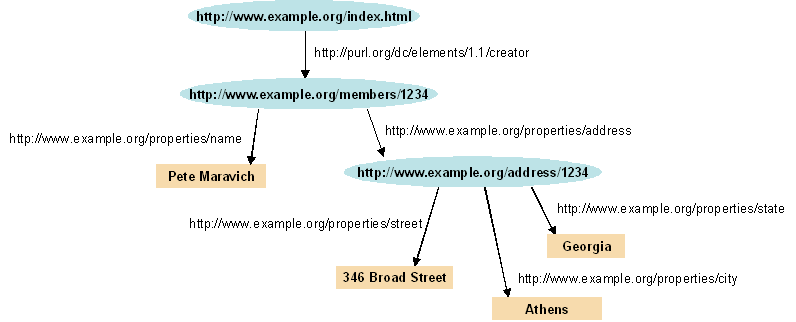
\includegraphics[width=\linewidth]{rdf.png}
	\caption{Example of RDF representation of an address}
	\label{fig:rdfGraph}
\end{figure}

Several methods exist for serializing the RDF data model. The most common format is RDF/XML. There exist other text-based formats introduced by W3C such as Turtle\footnote{\url{http://www.w3.org/TeamSubmission/turtle}} and N-Triples\footnote{\url{http://www.w3.org/TR/n-triples}} which are easier to read than RDF/XML.

RDF also contains data structures (containers and collections) that allow aggregating nodes or facts together. They are basically a syntactic sugar that will ease the process of writing code with no semantic expressiveness whatsoever.

\subsection{RDF Schema}

\begin{flushright}
	\textit{``It's impossible to get everyone everywhere to agree on a single label for every specific thing that ever was, is, or shall be''}\\
	Cambridge Semantics~\cite{Cambridge:RDF-101:13}
\end{flushright}

RDF is a simple and flexible data model that describes resources using properties and values. Predicates in RDF are what describe and give meaning to statements. They act as a vocabulary or an ontology. An ontology is an explicit specification of a conceptualization~\cite{Gruber:KA:93}. It is a formal way to organize knowledge and terms and reflect common understanding of a domain. Ontologies are typically represented as graphical relationships or networks as opposed to taxonomies which are usually presented hierarchically. Some core elements of an ontology are:

\begin{itemize}
	\item Class: defines a concept, type or collection within a specific domain. It encapsulates objects sharing some properties. For instance, in a geographical domain, the class Country is more specialized than the class Place.
	\item Individual: also known as instance or object and is a member of a class. For instance, \emph{France} is an instance of the class Country.
	\item Property: is a binary relation describing how classes and individuals relate to each other. A datatype property connects instances with RDF literals while object property connects instances of two classes. For example, \emph{hasCity} is an object property that can relate two instances of the class City.
\end{itemize}

In order for Semantic Web applications to be able to share data, they must agree on common vocabulary. RDF doesn't provide ways to define those vocabularies and to specify domain specific classes and properties. To overcome this limitation, an extension of RDF called RDF Schema (RDFS)~\cite{Brickley:RDFS:14} provides a basic vocabulary to interpret RDF statements, describe taxonomies of classes and properties and define very basic restrictions.

RDFS as a modeling language allows for: 1) definition of classes and their instantiation, 2) definition of properties and restrictions and 3) definition of hierarchies for classes and properties.

\begin{itemize}
	\item Resources are instances of one or more class (\emph{rdfs:class}). Classes are organized in a hierarchy using~\emph{rdfs:subClassOf} property.
	\item Properties are assigned the class \emph{rdf:Property} and are organized in a hierarchy using~\emph{rdfs:subPropertyOf}.
	\item Restrictions on properties can be specified. For example,~\emph{rdfs:domain} to define the class of the subject and \emph{rdfs:range} to define the class of the object.
\end{itemize}

\subsection{Web Ontology Language}

RDFS provides basic hierarchies associated with simple restrictions. This limited expressivity triggered the need to define an explicit formal description of concepts in complex domains. As a result, the Web Ontology Language (OWL)~\cite{W3C:OWL:12} which adds more vocabulary for describing properties and classes on top of RDF is the current markup language endorsed by W3C. It provides more relations between classes (e.g., \emph{disjointWith}), logical properties (e.g., \emph{intersectionOf}, \emph{sameAs}) and enumerations (e.g., \emph{oneOf}, \emph{allValuesFrom}), among others.

\subsection{SPARQL Query Language}

Relational databases can be efficient for semantic databases. However, in practice, they are designed for a different type of workload. The fundamental operation of semantic databases is join, which is naturally expensive in relational databases. Given that we have our data modeled as RDF regardless of the underlying database choice, it is now possible to query and ask questions about our data in a very powerful way. Protocol and RDF Query Language (SPARQL)~\cite{Prud:SPARQL:08} is the standardized query language for RDF.

A SPARQL query consists of a set of triples where each part (subject, predicate and/or object) can consist of variables alongside a set of conjunctions (e.g., logical ``and'') or disjunctions (e.g., logical ``or''). It works by matching the triples in the query with the existing RDF triples and resolving the variables.

\subsection{Linked Data}

The traditional approach of sharing data through independent silos is diminishing with the various advances in the Web. The Semantic Web envisages the availability of large amount of interlinked RDF data. Linked Data (LD) is a major milestone towards achieving this vision. Formally, Linked Data has been defined as about ``data published on the Web in such a way that it is machine readable, its meaning is explicitly defined, it is linked to other external datasets, and can in turn be linked to from external datasets''~\cite{Bizer:IJSWIS:09}.

\begin{figure}[ht!]
	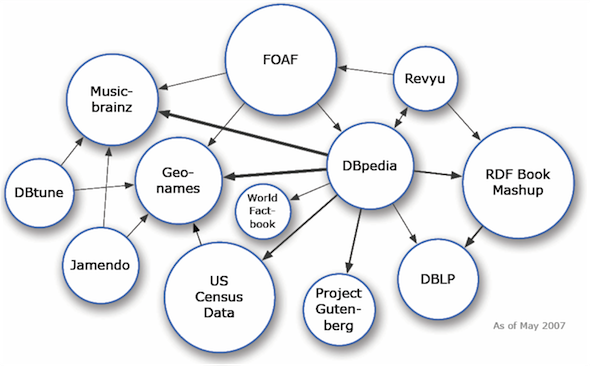
\includegraphics[width=0.9\textwidth]{lod-cloud2007.png}
	\caption{The LOD cloud as of May, 2007}
	\label{fig:lodcloud2007}
\end{figure}

Linked Data follows four main principles outlined by Tim Berners-Lee~\cite{Berners-Lee:W3C:06} to publish information on the Web, which are:

\begin{enumerate}
	\item Use URIs as names for things
	\item Use HTTP URIs so that people can look up those names
	\item When someone looks up a URI, provide useful information, using the standards (RDF, SPARQL)
	\item Include links to other URIs. so that they can discover more things
\end{enumerate}

Linked Data is continuously evolving, started in 2007 with a dozen of datasets (see Figure~\ref{fig:lodcloud2007}) to reach today thousands of datasets covering knowledge from various domains such as encyclopedic, government, geographic, entertainment and so on. The datasets have tripled in size from 2011 to 2014, with a significant growth of nearly $271\%$~\cite{Schmachtenberg:ISWC:14}. The latest version published in April 2014 contains 1014 linked datasets connected by 2909 linksets (see Figure~\ref{fig:lodcloud2014}).

One of the most widely used datasets is DBpedia\footnote{http://dbpedia.org}. It is a structured knowledge extracted from multilingual versions of Wikipedia~\cite{Bizer:WebSemJorunal:09}. At the time of writing, the English version of DBpedia consists of 470 millions RDF triples that describe 4.0 million things covering a wide range of topics, and contains 45 million RDF links to several hundred external datasets.

In order to achieve the Linked Data vision, datasets should contain outbound links to other datasets. Significant efforts try to automatically or semi-automatically generate these link to facilitate data discovery and to attach additional information.

\section{Open Data}\label{section:openData}

Open Data (OD) is the data that can be easily discovered, accessed, reused and redistributed by anyone~\cite{Davies:Report:15}. Open data has both legal and technical dimensions. It is placed in the public domain under liberal terms of use with minimal restrictions and is available in electronic formats that are non-proprietary and machine readable.

Businesses, citizens and governments are encouraged to publish, share and reuse data. Figure~\ref{fig:opendata_ecosystem} shows the Open Data ecosystem described by~\cite{Deloitte:Report:12}. Each party in this ecosystem supplies different types of data (e.g., Open Business Data (OBD), Open Government Data (OGD)) to different types of stakeholders.

\begin{figure}[ht!]
	\centering{
	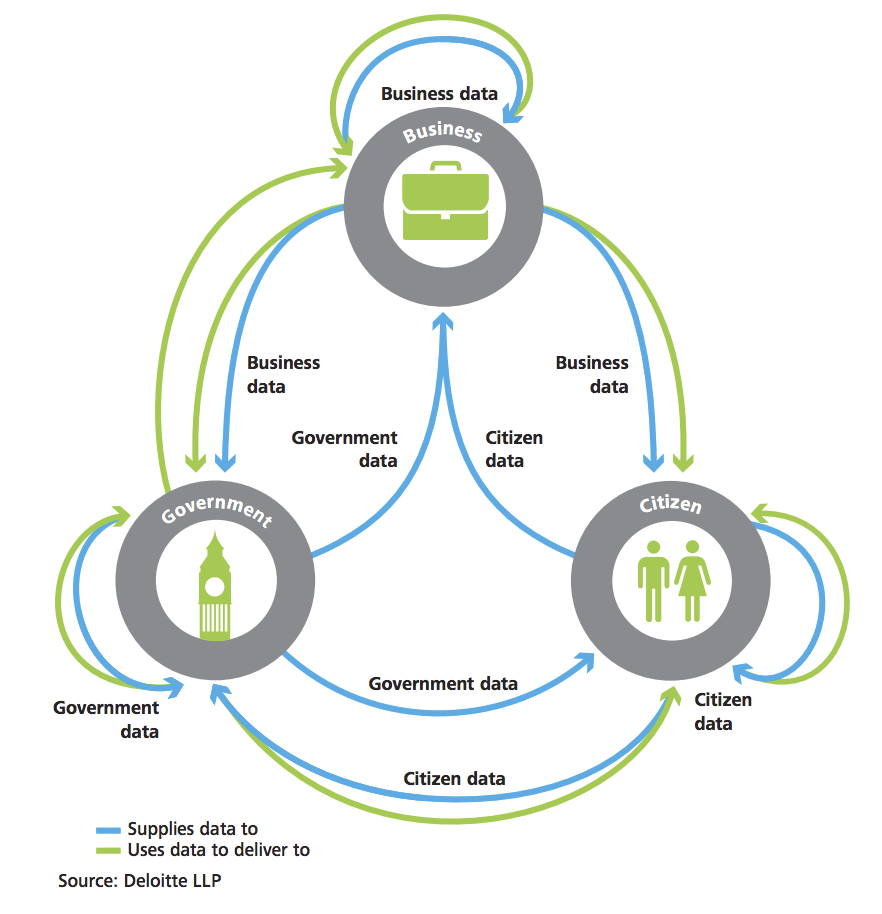
\includegraphics[width=0.6\textwidth]{opendata_ecosystem.png}
	\caption{Open Data ecosystem}
	\label{fig:opendata_ecosystem}
	}
\end{figure}

Linked Open Data refers to the semantically linked, machine-readable open data. Tim Berners-Lee~\cite{Berners-Lee:W3C:06} outlined a 5 starts scheme to evaluate the availability of Linked Data as Linked Open Data:

\begin{enumerate}
	\item Data available on the web in any format, even using PDF or image scan, but with an open license
	\item Data delivered as machine-readable structured data, e.g., excel instead of image scan of a table
	\item Data available in a non-proprietary format, e.g., CSV instead of Excel
	\item All the above plus, data using open standards from W3C, e.g., RDF and SPARQL, to identify things and properties, so that people can point at other data
	\item All the above, plus, to link data to other people's data to provide context
\end{enumerate}

Open Data has major benefits for citizens, businesses, societies and governments. It increases transparency and enables self-empowerment by improving the visibility of previously inaccessible information; allowing citizens to be better informed about policies, public spending and activities in the law making processes~\cite{Deloitte:Report:12, Manyika:Report:13}.

Open Data is considered a gold mine for organizations which are trying to leverage external data sources in order to produce more informed business decisions~\cite{Boyd:Article:11}. Despite the legal issues surrounding Open Data licenses~\cite{Prateek:Misc:13}, McKinsey~\cite{Manyika:Report:13} estimates that Open Data in the health sector alone adds up over \$300 billion to the economy every year.

These huge benefits led to a world-wide adoption of Open Data. Figure~\ref{fig:god_adoption} shows the existence and support for open data initiatives, engagement with open data from outside government, legislative frameworks that support open data and the existence of training and support for data use and innovation~\cite{Davies:Report:15}.
Moreover, there are several reports and initiatives like Open Data Barometer\footnote{\url{http://barometer.opendataresearch.org/}}, Open Data Monitor\footnote{\url{http://opendatamonitor.eu}} and Global Open Data Index\footnote{\url{http://index.okfn.org/}}that aim at analyzing and monitoring the adoption of Open Data across the world.

Going back to our scenario in~\ref{section:scenario}, Open Data will help our analyst \textbf{Dan} in:

\begin{itemize}
	\item Having a transparent view on the data available by Ministry of Transport in France. This helps in preventing the possibility of wasting time and funds recollecting data that has been already collected by a different department.
	\item Discovering complementary datasets from other sources. The benefits of data transparency amplifies when it is widely adopted in all other departments and agencies.The additional data enrich reports and enable better-informed, data-driven decisions. For example, by providing extra details on traffic information at the time when accidents occurred, \textbf{Dan} could draw more accurate conclusions on the root cause of some of these accidents.
\end{itemize}

\begin{figure}[ht!]
	\centering{
	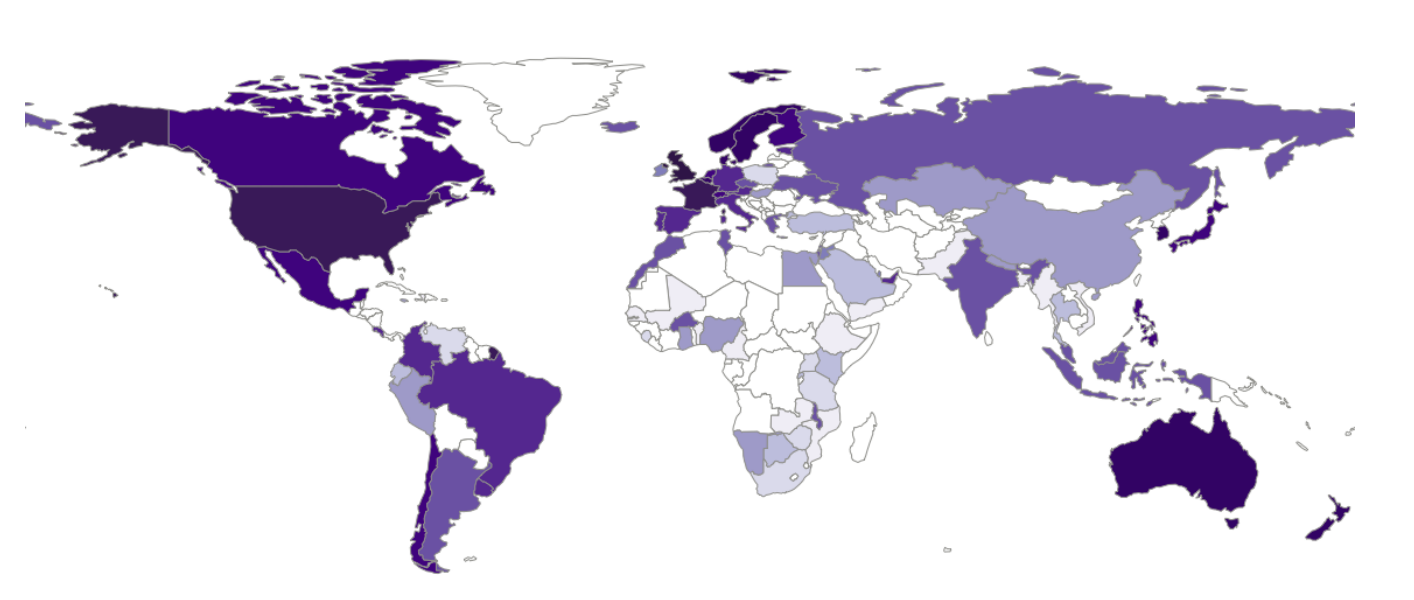
\includegraphics[width=0.9\textwidth]{god_adoption.png}
	\caption{Heat map of Open Government Data adoption according to the Open Data Barometer 2015}
	\label{fig:god_adoption}
	}
\end{figure}

\subsection{Open Licenses}

Project Open Data~\footnote{https://project-open-data.cio.gov} emphasizes the importance of datasets reusability as one of the main principles for open data. Open data should be made available under an open license. This is of high importance specially for organizations looking to integrate data for commercial use. Figure~\ref{fig:lodcloud2014} shows the LOD cloud datasets licenses distribution. We notice that a considerable amount of datasets are still missing attached license information.

The Open Definition~\footnote{http://opendefinition.org/} defines a license as the legal conditions under which an item or piece of knowledge (also referred to as ``work'') is made available. Domain dedications like \emph{Creative Commons Zero} satisfy this definition although not technically a ``license''.

The Open Definition defines the following conditions for open licenses:

\begin{itemize}
	\item Allows free use of the work without any fee arrangement or compensation
	\item Allows redistribution (on its own or as part of a collection) of the work
	\item Allows distribution of modified work under the same license of the original
	\item Allows any part of the work to be freely used, distributed or modified separately
	\item Allows distribution of the work alongside other distinct works without placing restrictions on the additional ones
	\item Doesn't discriminate against any person or group
	\item Allows use, redistribution, modification, and compilation for any purpose
	\item Allows rights propagation to all to whom the work is distributed
\end{itemize}

\begin{figure}[ht!]
	\centering{
	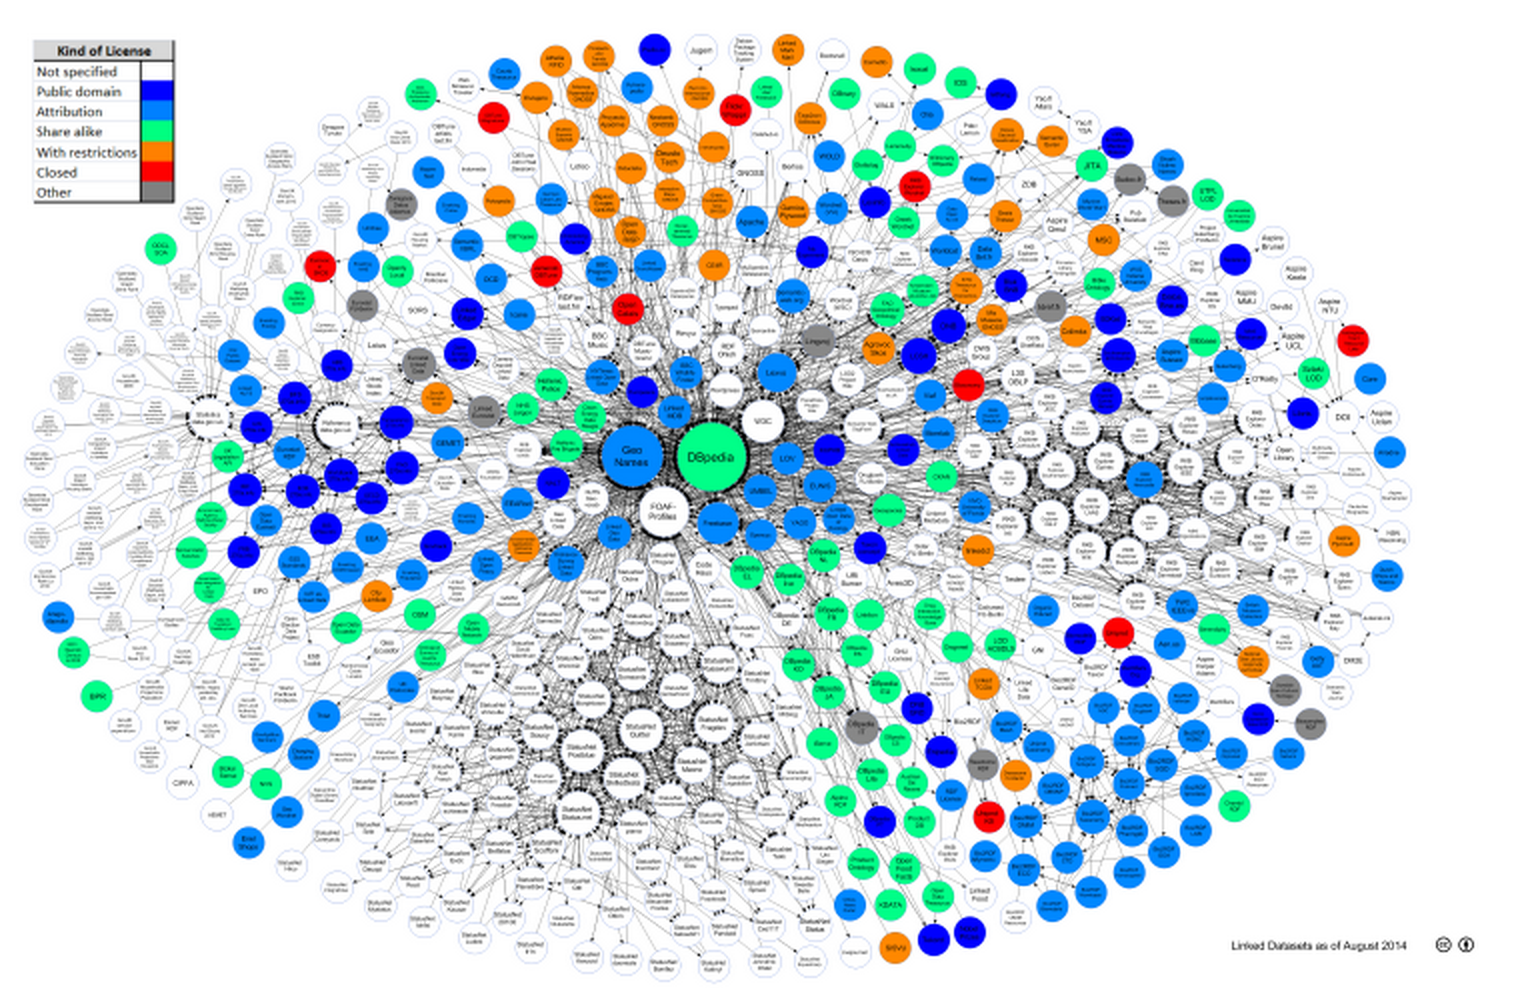
\includegraphics[width=0.9\textwidth]{lod14_licenses.png}
	\caption{Linking Open Data cloud diagram 2014, by Max Schmachtenberg, Christian Bizer, Anja Jentzsch and Richard Cyganiak colored by licensing types. \url{http://www.cosasbuenas.es/blog/how-o-is-lod-2015}}
	\label{fig:lodcloud2014}
	}
\end{figure}

Despite the legal issues surrounding Linked Data licenses~\cite{Prateek:Misc:13}, it is still considered a gold mine for organizations who are trying to leverage external data sources in order to produce more informed business decisions~\cite{Boyd:Article:11}. In~\cite{Manyika:Report:13}, the authors see the potential economic effect unfolding in education, transportation, consumer products, electricity, oil and gas, health care and consumer finance. They estimate the potential annual value enabled by Open Data in these domains to be 3 trillion US Dollars across seven domains.

\section{Data Profiling}\label{section:dataProfiling}

The huge amount of published data makes it difficult to discover relevant datasets through traditional inspection of the raw data. \textit{Data profiling} is the process of creating descriptive information and collect statistics about that data. It is a cardinal activity when facing an unfamiliar dataset~\cite{Li:WISM:12, Kimball:DWL:98}.

Data profiling is a vital task to monitor the quality of internal data in the enterprise. Halo BI report~\cite{Halo:TechReport:13} states that nearly 40\% of company's data is found to be inaccurate. 25\% of which is considered critical data.

Data profiles reflect the importance of datasets without the need for detailed inspection of the raw data.  It also helps in assessing the importance of the dataset, improving users' ability to search and reuse part of the dataset and detecting irregularities to improve its quality. Data profiling includes typically several tasks:
\begin{itemize}
  \item \textbf{Metadata profiling}: Provides general information on the dataset (dataset description, release and latest update dates), legal information (license information, openness), practical information (access points, data dumps), etc.
  \item \textbf{Statistical profiling}: Provides statistical information about data types and patterns in the dataset (e.g., properties distribution, number of entities and RDF triples).
  \item \textbf{Topical profiling}: Provides descriptive knowledge on the dataset content and structure. This can be in form of tags and categories used to facilitate search and reuse.
  \item \textbf{Quality profiling}: Discovers inconsistencies and anomalies in the data. Data is considered of high quality if is appropriate for use and if it correctly represents the world constructs to which it refers~\cite{Juran:McGraw:99}.
\end{itemize}

Dataset profiles are collections of data describing the internal structure of the dataset. They are presented as a set of metadata in different formats such as JSON, XML and RDF. The Linked Data publishing best practices~\cite{Bizer:DB:11} specifies that datasets should contain metadata needed to effectively understand and use them. Metadata is structured information that describes, explains, locates, or otherwise makes it easier to retrieve, use, or manage an information resource~\cite{NISO:TechReport:04}. Having rich metadata helps in enabling:
\begin{itemize}
  \item \textbf{Data discovery, exploration and reuse}: In~\cite{Graham:TechReport:11}, it was found that users are facing difficulties finding and reusing publicly available datasets. Metadata provides an overview of datasets making them more searchable and accessible. High quality metadata can be at times more important than the actual raw data especially when the costs of publishing and maintaining such data is high.
  \item \textbf{Organization and identification}: The increasing number of datasets being published makes it hard to track, organize and present them to users efficiently. Attached metadata helps in bringing similar resources together and distinguish useful links.
  \item \textbf{Archiving and preservation}: There is a growing concern that digital resources will not survive in usable forms to the future~\cite{NISO:TechReport:04}. Metadata can ensure resources survival and continuous accessibility by providing clear provenance information to track the lineage of digital resources and detail their physical characteristics.
\end{itemize}

\section{Conclusion}

In this chapter, we set up the grounds for the rest of this part of the thesis. We presented that basic concepts in semantic Web, open and linked data as well as data profiling and its subtasks.